\section{Cơ sở lý thuyết}
\subsection{Tụ điện}
\subsubsection{Cấu tạo}
Một tụ điện (capacitor) gồm có 2 vật dẫn như hình vẽ. Các vật dẫn này được gọi là các
bản tụ (plate). Khi vật dẫn được tích điện, các bản tụ sẽ mang điện tích bằng nhau về độ
lớn nhưng ngược dấu. Hiệu điện thế tồn tại giữa các bản tụ gây ra bởi các điện tích.

\begin{figure}[H]
    \centering
    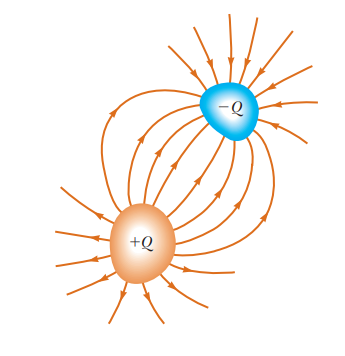
\includegraphics[width=0.4\linewidth]{images/figure1.png}
    \caption{Biểu diễn sơ đồ điện trường của một tụ điện bất kỳ, gồm hai vật dẫn mang điện lượng bằng nhau nhưng trái dấu ($+Q$ và $-Q$)}
    \label{fig:placeholder}
\end{figure}

\subsubsection{Định nghĩa}
Khi vật dẫn $B$ bao trùm hết vật dẫn $A$, ta tích cho vật dẫn $A$ một điện tích $+Q$, thì hai bề mặt trong và ngoài của vật dẫn $B$ sẽ tích điện $-Q$, $+Q$. Nối mặt ngoài cùng của vật dẫn $B$ xuống đất (mặt ngoài cùng trung hòa) ta có hai bề mặt kim loại tích điện trái dấu $-Q$, $+Q$ gọi là hai bản (cốt) của tụ điện.

\begin{figure}[H]
    \centering
    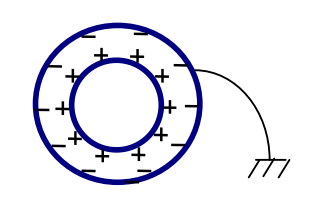
\includegraphics[width=0.5\linewidth]{images/figure2.png}
    \caption{Mô hình cấu tạo tụ điện: Vật dẫn bao ngoài được nối đất để triệt tiêu điện tích cùng dấu, tạo thành hai bản tụ mang điện tích trái dấu có độ lớn bằng nhau.}
    \label{fig:placeholder}
\end{figure}

\subsubsection{Điện dung của tụ điện}
Khi ta tích điện cho một tụ điện điện lượng $Q$, giữa hai bản tụ sẽ xuất hiện một hiệu điện thế $\Delta V$. Nếu tiếp tục tăng điện tích $Q$ thì hiệu điện thế $\Delta V$ cũng tăng theo tỉ lệ thuận tương ứng. Tuy nhiên, tỉ số giữa độ lớn điện tích $Q$ và hiệu điện thế $\Delta V$ luôn luôn là một hằng số đối với một tụ điện nhất định.

Hằng số này đặc trưng cho khả năng tích điện của tụ điện ở một hiệu điện thế cho trước, và được gọi là điện dung của tụ điện.

Biểu thức định nghĩa điện dung: 
$$C = \frac{Q}{\Delta V}$$

Trong đó: 
\begin{itemize}
\item $C$: Điện dung của tụ điện, có đơn vị là Farad (F).
\item $Q$: Độ lớn điện tích trên một bản tụ, có đơn vị là Coulomb (C).
\item $\Delta V$: Hiệu điện thế giữa hai bản tụ, có đơn vị là Volt (V).
\end{itemize}

\subsubsection{Tụ điện phẳng}
\begin{figure}[H]
    \centering
    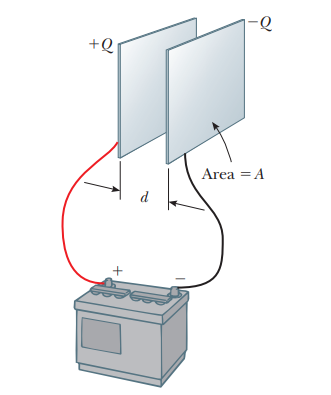
\includegraphics[width=0.4\linewidth]{images/figure3.png}
    \caption{Cấu tạo cơ bản của tụ điện phẳng: Hai bản kim loại có cùng diện tích bề mặt $A$, đặt cách nhau một khoảng $d$ và mang điện lượng trái dấu ($+Q$ và $-Q$) khi được nạp điện.}
    \label{fig:placeholder}
\end{figure}
Tụ điện phẳng là một trong những cấu trúc cơ bản và mang tính nền tảng nhất trong nghiên cứu tĩnh điện học. Cấu tạo không gian của hệ thống này bao gồm hai bản kim loại phẳng có cùng diện tích bề mặt $A$, được bố trí song song với nhau và ngăn cách bởi một khoảng cách $d$ trong môi trường chân không (hoặc không khí). Quá trình nạp điện cho hệ thống dẫn đến sự phân bố điện tích đối xứng, trong đó một bản mang điện tích dương $+Q$ và bản đối diện mang điện tích âm $-Q$. Hệ quả của quá trình này là sự hình thành mật độ điện tích mặt $\sigma$ trên bề mặt mỗi bản kim loại, được xác định bởi tỷ số giữa lượng điện tích và diện tích bề mặt tương ứng:
$$\sigma = \frac{Q}{A}$$

Trong các khảo sát lý thuyết, một giả thiết lý tưởng hóa thường được áp dụng là khoảng cách $d$ rất nhỏ so với kích thước tuyến tính của các bản tụ. Giả thiết này đóng vai trò quan trọng trong việc loại bỏ ảnh hưởng của hiệu ứng mép tại các rìa vật dẫn, cho phép xem xét điện trường $\vec{E}$ nội bộ giữa hai bản tụ là một điện trường đều, đồng thời coi điện trường ở không gian bên ngoài hệ thống xấp xỉ bằng $0$. Dựa trên cơ sở đó và thông qua việc áp dụng định lý Gauss, độ lớn của cường độ điện trường đều bên trong khoảng không gian giữa hai bản tụ được xác định chặt chẽ bằng biểu thức:
$$E = \frac{\sigma}{\epsilon_0} = \frac{Q}{\epsilon_0 A}$$
\textit{(Với $\epsilon_0$ là hằng số điện của chân không).}

Do đặc tính phân bố đều của điện trường nội bộ, độ giảm thế (hay hiệu điện thế $\Delta V$) giữa hai bản vật dẫn thể hiện mối quan hệ tuyến tính với chiều dài đường sức $d$. Mối liên hệ này được biểu diễn qua phương trình:
$$\Delta V = E \cdot d = \frac{Q \cdot d}{\epsilon_0 A}$$

Bằng cách tích hợp biểu thức hiệu điện thế này vào định nghĩa tổng quát của điện dung, biến số $Q$ được triệt tiêu, từ đó thiết lập được hệ thức toán học tính toán điện dung dành riêng cho cấu trúc tụ điện phẳng:
$$C = \frac{Q}{\Delta V} = \frac{\epsilon_0 A}{d}$$

Việc thiết lập phương trình giải tích trên đã minh chứng cho một nguyên lý vật lý cốt lõi: điện dung của một tụ điện phẳng mang tính chất nội tại và hoàn toàn độc lập với lượng điện tích $Q$ mà hệ đang lưu trữ hay hiệu điện thế $\Delta V$ được áp đặt lên nó. Thực chất, đại lượng này được quyết định hoàn toàn bởi các thông số cấu trúc không gian của hệ thống - tỷ lệ thuận với diện tích bề mặt bản tụ $A$, tỷ lệ nghịch với khoảng cách $d$ - và bản chất của môi trường điện môi tồn tại giữa hai bản cực.

\subsubsection{Sự phụ thuộc của điện dung vào các yếu tố hình học}
Từ biểu thức tính điện dung của tụ điện phẳng ($C = \frac{\epsilon_0 A}{d}$), ta có thể giải thích bản chất vật lý của sự phụ thuộc này thông qua các đặc điểm sau:
\begin{enumerate}
    \item Ảnh hưởng của diện tích bản tụ ($A$)\\
    Khi tụ điện được nạp điện từ một nguồn, các electron sẽ di chuyển và tích tụ trên bản cực âm, đồng thời bản cực dương mất đi một lượng electron tương ứng. Nếu diện tích bề mặt bản tụ $A$ càng lớn, không gian để điện tích phân bố càng rộng rãi. Điều này cho phép các bản tụ chứa được một lượng điện tích lớn hơn nhiều mà vẫn duy trì cùng một mức hiệu điện thế. Do đó, điện dung của tụ điện tỉ lệ thuận với diện tích bề mặt bản tụ ($C \propto A$).
    \item Ảnh hưởng của khoảng cách giữa hai bản tụ ($d$)\\
    Xét trường hợp tụ điện đang được duy trì kết nối với một nguồn điện (pin). Giả sử ta dịch chuyển để đưa hai bản tụ lại gần nhau (làm giảm khoảng cách $d$).
    \begin{itemize}
        \item Ngay tại khoảnh khắc dịch chuyển, lượng điện tích trên các bản tụ chưa kịp thay đổi tức thời, do đó cường độ điện trường $E$ giữa hai bản tạm thời giữ nguyên.
        \item Tuy nhiên, vì khoảng cách $d$ giảm, hiệu điện thế giữa hai bản tụ lúc này (tính theo công thức $\Delta V = E \cdot d$) sẽ bị suy giảm, trở nên nhỏ hơn hiệu điện thế của nguồn pin.
    \end{itemize}
\end{enumerate}

Sự chênh lệch điện áp này ngay lập tức tạo ra một điện trường dọc theo các dây nối, thúc đẩy dòng điện tích tiếp tục di chuyển từ nguồn vào tụ điện. Quá trình này làm tăng lượng điện tích $Q$ trên các bản tụ, kéo theo sự gia tăng hiệu điện thế giữa chúng. Dòng điện tích sẽ chỉ dừng lại khi hiệu điện thế của tụ điện phục hồi và cân bằng hoàn toàn với hiệu điện thế của pin.

Như vậy, thao tác đưa hai bản cực lại gần nhau đã giúp tụ điện gia tăng khả năng tích trữ điện tích ở cùng một mức điện áp. Ngược lại, nếu khoảng cách $d$ tăng lên, lượng điện tích lưu trữ sẽ giảm đi. Điều này giải thích bản chất vật lý của mối quan hệ tỉ lệ nghịch giữa điện dung $C$ và khoảng cách $d$ ($C \propto \frac{1}{d}$).

\subsection{Cường độ điện trường trong tụ điện phẳng}
\subsubsection{Định lý Gauss}
Định lý Gauss trong tĩnh điện học phát biểu rằng: Thông lượng điện trường gửi qua một mặt kín bất kỳ (gọi là mặt Gauss) bằng tổng đại số các điện tích nằm trọn bên trong mặt đó chia cho hằng số điện của chân không.

Biểu thức toán học:
$$\Phi_E = \oint \vec{E} \cdot d\vec{A} = \frac{q_{in}}{\epsilon_0}$$

Trong đó:
\begin{itemize}
    \item $\Phi_E$: Thông lượng điện trường qua mặt kín.
    \item $\vec{E}$: Vectơ cường độ điện trường tại vị trí vi phân diện tích.
    \item $q_{in}$: Tổng đại số các điện tích được bao bọc bên trong mặt Gauss.
    \item $\epsilon_0$: Hằng số điện của chân không.
\end{itemize}

Nguyên tắc chọn mặt Gauss:

Mặc dù định lý Gauss đúng với mọi mặt kín, nhưng trong thực hành, để tính toán cường độ điện trường $\vec{E}$ một cách dễ dàng, ta cần chọn một mặt Gauss phù hợp dựa trên tính đối xứng của sự phân bố điện tích. Bề mặt được chọn cần thỏa mãn ít nhất một trong các điều kiện sau đây để đơn giản hóa quá trình lấy tích phân:
\begin{enumerate}
    \item \textbf{Tính đối xứng về độ lớn:} Độ lớn cường độ điện trường $E$ không đổi tại mọi điểm trên bề mặt.
    \item \textbf{Điện trường vuông góc với mặt phẳng:} Vectơ điện trường $\vec{E}$ song song với vectơ diện tích $d\vec{A}$. Khi đó, biểu thức dưới dấu tích phân trở thành vô hướng: $\vec{E} \cdot d\vec{A} = E dA$.
    \item \textbf{Điện trường tiếp tuyến với mặt phẳng:} Vectơ điện trường $\vec{E}$ vuông góc với vectơ diện tích $d\vec{A}$. Khi đó, tích vô hướng triệt tiêu: $\vec{E} \cdot d\vec{A} = 0$.
    \item \textbf{Vùng không có điện trường:} Cường độ điện trường bằng không tại mọi điểm trên bề mặt xét ($E = 0$).
\end{enumerate}


\subsubsection{Xác định cường độ điện trường bằng định lý Gauss}
Để xác định cường độ điện trường trong tụ điện phẳng, quy trình tính toán được thực hiện qua hai giai đoạn: xác định điện trường do một bản phẳng đơn lẻ gây ra và áp dụng nguyên lý chồng chất cho hệ hai bản tụ.

\textbf{Cường độ điện trường của một bản phẳng tích điện}
    
Xét một bản kim loại phẳng vô hạn, tích điện đều với mật độ điện tích mặt $\sigma$. Chọn mặt Gauss là một hình trụ có trục vuông góc với bản tích điện và hai đáy song song với bản đó. Do tính đối xứng, vectơ cường độ điện trường $\vec{E}$ có hướng vuông góc với bản kim loại và độ lớn bằng nhau tại mọi điểm trên hai mặt đáy của hình trụ. Trong khi đó, thông lượng điện trường qua mặt xung quanh của hình trụ bằng không vì các đường sức song song với bề mặt này.

Áp dụng định lý Gauss, thông lượng điện trường chỉ đi qua hai mặt đáy, dẫn đến biểu thức xác định cường độ điện trường do một bản phẳng gây ra có độ lớn:
$$E = \frac{\sigma}{2\epsilon_0}$$

\textbf{Cường độ điện trường bên trong và bên ngoài tụ điện}

Xét mô hình tụ điện phẳng gồm hai bản kim loại song song mang điện tích trái dấu với mật độ $\sigma$ và $-\sigma$. Theo nguyên lý chồng chất, cường độ điện trường tại một điểm bất kỳ là tổng vectơ của điện trường do từng bản cực tạo ra.

\begin{itemize}
    \item \textbf{Vùng không gian giữa hai bản tụ:} Các vectơ điện trường do bản dương và bản âm gây ra có cùng phương và cùng hướng. Do đó, chúng cộng đại số với nhau, tạo ra điện trường bên trong tụ điện có độ lớn không đổi:
    $$E = \frac{\sigma}{2\epsilon_0} + \frac{\sigma}{2\epsilon_0} = \frac{\sigma}{\epsilon_0}$$
    \item \textbf{Vùng không gian bên ngoài tụ điện:} Vectơ điện trường do hai bản cực gây ra có cùng độ lớn nhưng ngược chiều nhau. Hệ quả là chúng triệt tiêu lẫn nhau, khiến cường độ điện trường ở vùng này xấp xỉ bằng không.
\end{itemize}

\textbf{Điều kiện áp dụng mô hình lý tưởng}

Các kết quả phân tích trên được thiết lập dựa trên mô hình tụ điện lý tưởng, trong đó thỏa mãn các điều kiện sau: diện tích của hai bản tụ đủ lớn để có thể coi là vô hạn, khoảng cách $d$ giữa hai bản rất nhỏ so với kích thước tuyến tính của chúng, và có thể bỏ qua hiệu ứng mép tại các rìa bản tụ.

\subsection{Năng lượng và mật độ năng lượng điện trường}
Việc tách biệt các điện tích dương và âm trong hệ thống hai vật dẫn của tụ điện đòi hỏi một công cơ học nhất định. Công này không mất đi mà được lưu trữ trong hệ thống dưới dạng năng lượng tiềm tàng, cụ thể là năng lượng tĩnh điện. Khi tụ điện được phóng điện thông qua một dây dẫn, năng lượng này sẽ được giải phóng, đôi khi có thể quan sát được dưới dạng tia lửa điện hoặc gây ra hiện tượng giật điện nếu tiếp xúc trực tiếp.

\begin{figure}
    \centering
    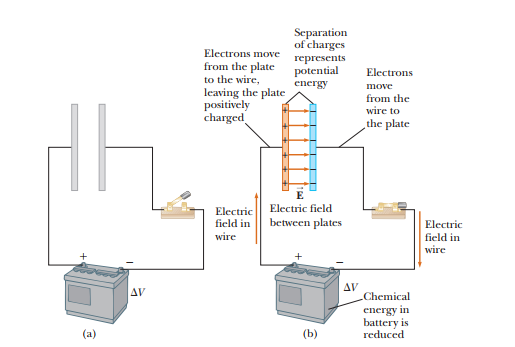
\includegraphics[width=0.7\linewidth]{images/figure4.png}
    \caption{Sơ đồ mô tả quá trình nạp điện và chuyển hóa năng lượng trong tụ điện phẳng: (a) Khi mạch hở; (b) Khi đóng công tắc, năng lượng hóa học từ pin chuyển hóa thành năng lượng điện thế thông qua sự phân tách các điện tích và thiết lập điện trường $\vec{E}$ giữa hai bản tụ.}
    \label{fig:placeholder}
\end{figure}
\subsubsection{Tính toán năng lượng lưu trữ trong tụ điện}
Để xác định tổng năng lượng tích lũy, ta xem xét quá trình nạp điện cho tụ điện như một chuỗi các bước dịch chuyển điện tích vi phân. Giả sử tại một thời điểm bất kỳ trong quá trình nạp, điện tích trên tụ điện là $q$ và hiệu điện thế tương ứng là $\Delta V$. Theo định nghĩa về điện dung, ta có mối liên hệ:
$$\Delta V = \frac{q}{C}$$

Khi một lượng điện tích vi phân $dq$ được chuyển từ bản mang điện thế thấp sang bản mang điện thế cao hơn, công vi phân $dW$ cần thực hiện để thắng lực điện trường là:
$$dW = \Delta V dq = \frac{q}{C}dq$$

Tổng công cần thiết để nạp điện cho tụ điện từ trạng thái không tích điện ($q=0$) đến khi đạt điện tích cuối cùng $Q$ được xác định bằng phép tính tích phân:
$$W = \int_{0}^{Q} \frac{q}{C} dq = \frac{1}{C} \int_{0}^{Q} q \, dq = \frac{Q^2}{2C}$$

\begin{figure}[H]
    \centering
    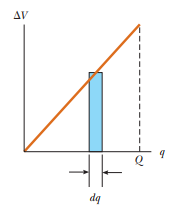
\includegraphics[width=0.35\linewidth]{images/figure5.png}
    \caption{Mối liên hệ tuyến tính giữa hiệu điện thế và điện tích của tụ điện. Tổng công thực hiện để nạp điện cho tụ đạt giá trị $Q$ tương ứng với diện tích hình tam giác nằm dưới đường thẳng $\Delta V(q)$.}
    \label{fig:placeholder}
\end{figure}

Vì công thực hiện bằng với năng lượng thế tĩnh điện $U$ tích lũy trong tụ điện, ta có các biểu thức tương đương để xác định năng lượng này:
$$U = \frac{Q^2}{2C} = \frac{1}{2}Q\Delta V = \frac{1}{2}C(\Delta V)^2$$

\subsubsection{Mật độ năng lượng điện trường}
Năng lượng trong tụ điện có thể được xem là lưu trữ trực tiếp trong điện trường tồn tại giữa hai bản cực. Đối với trường hợp tụ điện phẳng, ta có mối liên hệ giữa hiệu điện thế và cường độ điện trường là $\Delta V = Ed$, và điện dung $C = \frac{\epsilon_0 A}{d}$. Thay các giá trị này vào công thức năng lượng, ta thu được:
$$U = \frac{1}{2} \left( \frac{\epsilon_0 A}{d} \right) (Ed)^2 = \frac{1}{2} (\epsilon_0 Ad) E^2$$
Vì tích số $Ad$ chính là thể tích $V_{vol}$ của vùng không gian chứa điện trường, năng lượng trên mỗi đơn vị thể tích - gọi là mật độ năng lượng điện trường $u_E$ - được xác định như sau:
$$u_E = \frac{U}{Ad} = \frac{1}{2} \epsilon_0 E^2$$

Mặc dù biểu thức này được xây dựng dựa trên mô hình tụ điện phẳng, nó mang tính chất tổng quát và đúng cho bất kỳ điện trường nào trong chân không. Như vậy, mật độ năng lượng tại một điểm bất kỳ trong điện trường luôn tỷ lệ thuận với bình phương độ lớn cường độ điện trường tại điểm đó.

\subsection{Tụ điện phẳng có điện môi}
Chất điện môi là các vật liệu không dẫn điện, điển hình như cao su, thủy tinh hoặc giấy sáp. Việc đưa chất điện môi vào giữa các bản tụ không chỉ giúp ngăn cách vật lý giữa hai bản cực mà còn làm thay đổi đáng kể các đặc tính điện của hệ thống.
\subsubsection{Ảnh hưởng của điện môi lên điện dung}
\begin{figure}[H]
    \centering
    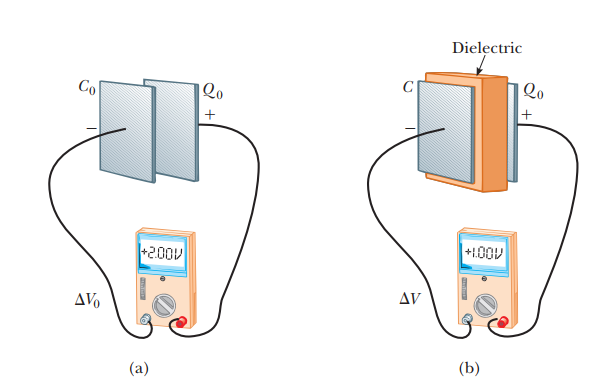
\includegraphics[width=0.6\linewidth]{images/figure6.png}
    \caption{Thí nghiệm minh họa ảnh hưởng của chất điện môi lên hiệu điện thế của tụ điện khi giữ nguyên điện lượng $Q_0$. (a) Hiệu điện thế ban đầu $\Delta V_0$ khi không có điện môi; (b) Hiệu điện thế $\Delta V$ giảm xuống sau khi chèn chất điện môi lấp đầy khoảng không gian giữa hai bản cực.}
    \label{fig:placeholder}
\end{figure}
Để khảo sát tác dụng của chất điện môi, xét một tụ điện phẳng đã được nạp điện lượng $Q_0$ và sau đó ngắt khỏi nguồn. Tại trạng thái ban đầu trong chân không, tụ điện có điện dung $C_0$ và hiệu điện thế đo được giữa hai bản tụ là $\Delta V_0 = Q_0/C_0$.

Khi chèn một tấm điện môi lấp đầy khoảng không gian giữa hai bản cực, thực nghiệm cho thấy hiệu điện thế giữa chúng giảm xuống một giá trị $\Delta V$ mới. Mối liên hệ giữa hiệu điện thế trước và sau khi có điện môi được xác định qua hệ số không thứ nguyên $\kappa$:
$$\Delta V = \frac{\Delta V_0}{\kappa}$$

Vì hệ thống đã được ngắt khỏi nguồn nên điện tích $Q_0$ trên các bản cực không thay đổi. Do đó, giá trị điện dung của tụ điện khi có điện môi phải thay đổi tương ứng:
$$C = \frac{Q_0}{\Delta V} = \frac{Q_0}{\Delta V_0 / \kappa} = \kappa \frac{Q_0}{\Delta V_0}$$
Hay:
$$C = \kappa C_0$$

Trong đó, $\kappa$ được gọi là hằng số điện môi của vật liệu. Vì thực nghiệm cho thấy $\Delta V < \Delta V_0$, ta luôn có $\kappa > 1$, nghĩa là việc chèn chất điện môi luôn làm tăng điện dung của tụ điện. Đối với mô hình tụ điện phẳng, biểu thức tính điện dung tổng quát khi có điện môi được xác định bởi:
$$C = \kappa \frac{\epsilon_0 A}{d}$$

\subsubsection{Giới hạn vật lý và điện áp định mức}
Mặc dù việc giảm khoảng cách $d$ hoặc tăng hằng số điện môi $\kappa$ có thể làm tăng điện dung, nhưng trong thực tế, các tham số này bị giới hạn bởi hiện tượng đánh thủng điện môi. Với mỗi loại vật liệu, tồn tại một giá trị cường độ điện trường tối đa mà nó có thể chịu đựng được trước khi mất tính cách điện và trở nên dẫn điện, gọi là độ bền điện môi.

Hệ quả là các tụ điện thực tế luôn đi kèm với thông số điện áp định mức (hoặc điện áp đánh thủng). Thông số này đại diện cho mức hiệu điện thế lớn nhất có thể đặt vào tụ điện mà không gây ra sự phóng điện xuyên qua lớp điện môi. Do đó, khi thiết kế và lựa chọn tụ điện cho các ứng dụng cụ thể, người kỹ sư cần phải xem xét đồng thời cả giá trị điện dung và giới hạn điện áp hoạt động để đảm bảo an toàn và độ bền cho hệ thống.
